\documentclass[11pt]{article}

\usepackage[margin=0.75in]{geometry}
\usepackage{indentfirst}
\usepackage{graphicx}
\usepackage{hyperref}
\usepackage{amsmath}

\bibliographystyle{siam}

\title{Appendix: Convolution Analysis}
\author{
  LeRoy, Benjamin\\
  \texttt{benjaminleroy}
}

\begin{document}
\maketitle


\section{Introduction}

fMRI data presents a distinct challenge for relating neural stimulation 
to BOLD (blood-oxygen-level dependent) response. fMRI scans record changes 
in oxygenation levels of hemoglobin in the brain. However, there is a delay 
between neural stimulation and the change in blood oxygen levels to a givein 
area. This delayed and lengthy response has been modeled using block stimulus 
and a classic example of this hemodyamic response function (with stimulation 
at t=0) can be seen in Figure \ref{fig:hrf}. The complete hemodynamic needs 
to be modeled in order to better relate  stimulation and the BOLD response 
from the fMRI.

\section{Mathematics}
\subsection{Convolution Theory/ Mathematics}

To relate stimuli to BOLD reponse, we convolved the time courses. At a basic 
level, convolution is a distinct combination of two functions (say $f$ and $g$).
 This combination is just the ``integral that expresses the amount of overlap of
  $f$ as it is shifted over another function $g$''  
  \cite{weissten2015convolution}. There are many examples of this, but the 
  following is basic idea that we'll expand of later. 

Let's define a function $f$ as a sum of 2 gamma functions, and $g$ as a 
``continous'' specialized step function  (we'll see why these functions are 
valuable later). Graphically we can see their plots in Figure \ref{fig:f}, 
\ref{fig:g}, and mathematically let's define them as follows as the following 
equation \ref{eq:gamma2} and \ref{eq:step} respectly.

\begin{equation} \label{eq:gamma2}
f(t)=\frac{.6}{.17}\cdot  \big[G_1(6,t)-.35 \cdot G_1(12,t) \big]
\end{equation}

where $G_1(k,t) =\frac{1}{\Gamma(k)} t^{k-1} e^{-t}$ (the gamma pdf with 
$\theta =1$)

\begin{equation} \label{eq:step}
 g(t)=\Big \{ \begin{tabular}{l c}
 		0  & if  5.85 $\leq$ t $\leq$ 6.15\\
 		.6  & otherwise \\
 		\end{tabular} \end{equation}
 		
 		
\begin{figure}[ht]
\centering
\begin{minipage}[b]{0.45\linewidth}
	\centering
	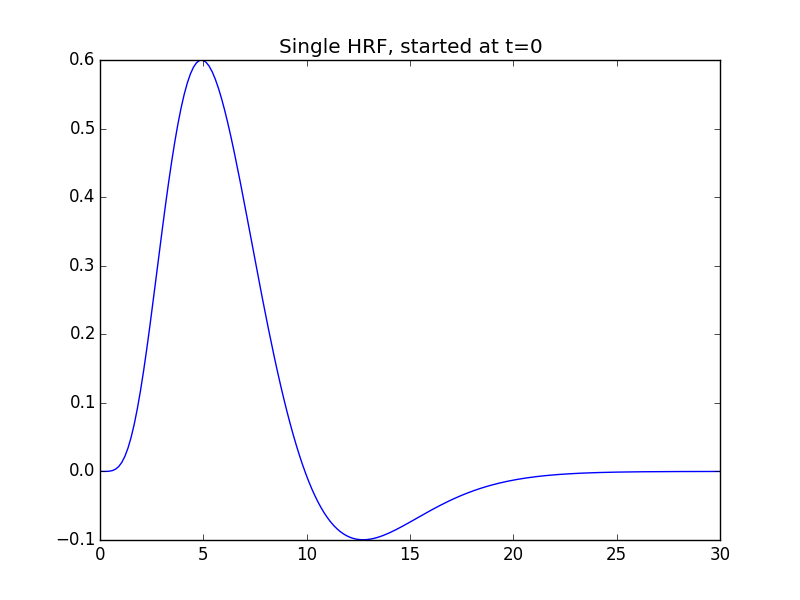
\includegraphics[width=.8\linewidth]{images/hrf_pattern.png} 
	\caption{$f$ (``Stablized Function'')}
	\label{fig:f}
\end{minipage}	
\quad
\begin{minipage}[b]{0.45\linewidth}
	\centering
		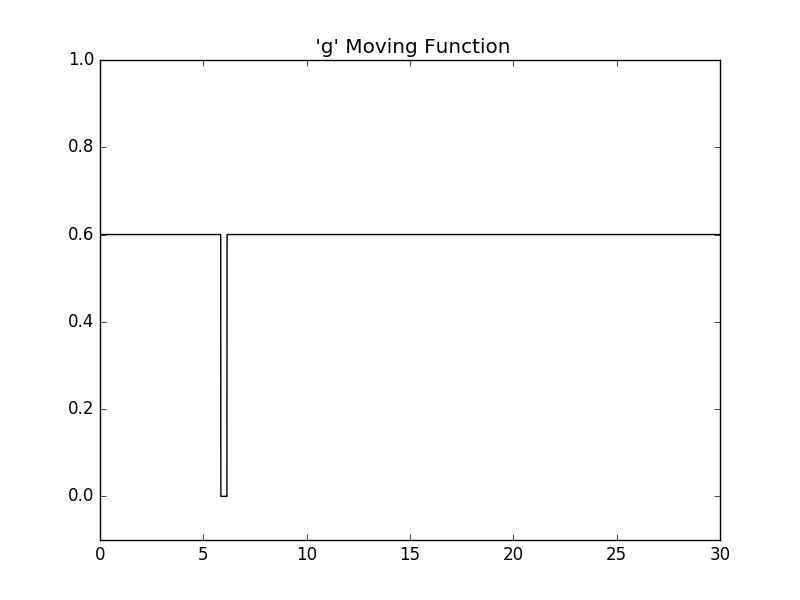
\includegraphics[width=.8\linewidth]{images/play.png} 
	\caption{$g$ (``Moving function'')}
	\label{fig:g}
\end{minipage}
\end{figure}


As mentioned in the basical level definition, if we move $g$ across $f$ from 
left to right, at discrete time intervals we'd see something similar to Figure 
\ref{fig:math}. If we plot these values (the integration of the differences), 
we'll get a plot very similar to f starting at a certain point.  **The plot 
actually cheats when $f$ is negative, and we'd have to alter definitions a 
little bit (will hopefully do later).**  If we had multiple bumps in our $g$ 
function ( i.e. multiple distinct``zero'' places'' we'd expect we'd get 
multiple non-zero differences between the functions at each time capture 
(this idea is needed later). 





\begin{figure}[ht]
	\centering
	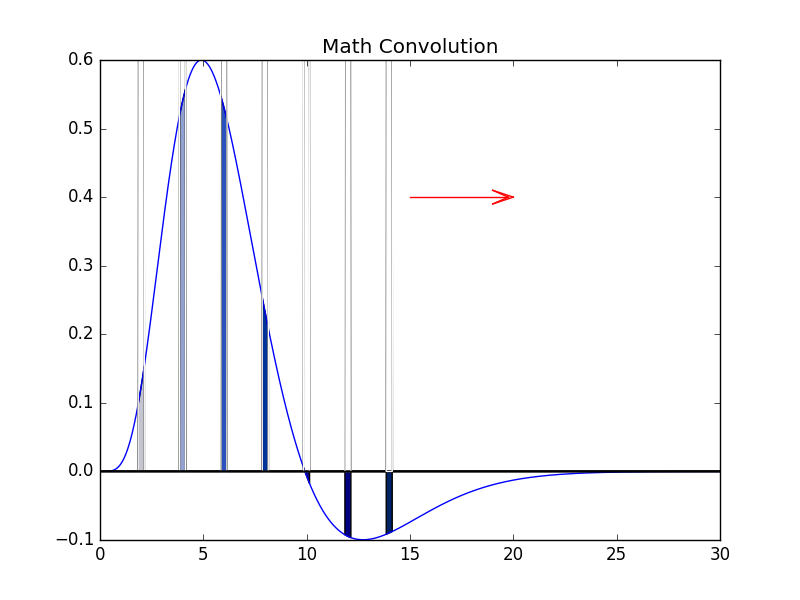
\includegraphics[width=.5\linewidth]{images/math_convolved.png}
	\caption{convolution of $f$ and $g$}
	\label{fig:math}
\end{figure}






\subsection{Convolution Applied to Stimulus}

The ``continous'' nature of the step function ``g'' doesn't extend well into 
discrete time series that we have. As such, and a very common change in fMRI 
analysis is to approach the convolution as something slightly different 
(through mathematical sums).  

For example in the previous section, we can treat $f$ as the same, and $g$ as 
$g'$ defined in equation \ref{eq:g_prime}.

\begin{equation}\label{eq:g_prime}
 g'(t)=\Big \{ \begin{tabular}{l c}
 		1  & if t=6\\
 		0  & otherwise \\
 		\end{tabular} \end{equation}

We could then define the value of the convolution of $g'$ and $f$ for discrete 
integers as in equation \ref{eq:math_discrete}.


\begin{equation}  \label{eq:math_discrete}
r(t)=  f(t-6)
\end{equation}



If we allow for multiple non-zero periods for $g'$ then we get a more general 
model in equation \ref{eq:math_discrete_extend}, where each $t_i$ is a value 
when $g'(t_i) \neq 0$

\begin{equation}  \label{eq:math_discrete_extend}
r(t)= \sum_{i=1}^n f(t-t_i)
\end{equation}

This equation gives a good glimpse into what a response of the hemodyamic 
response would be after stimulus at time $t_i$ for $i \in {1,...,n}$. Moreover 
you could extend the idea to including a ``strength'' value of the stimulus by 
changing the $g'|t_i$ to values other than 1, if that was the case we'd change 
the response equation to equation \ref{eq:math_discrete_final}. Equation 
\ref{eq:math_discrete_final} also allows us to include all discrete $t$ into 
the equation where $g'(t_i)$ now is expected to be zero (so $n$ becomes much 
larger). 

\begin{equation}  \label{eq:math_discrete_final}
r(t)= \sum_{i=1}^n g'(t_i) f(t-t_i)
\end{equation}


WIth this new equation we can look at function $f$ and $g'$ displayed 
graphically [Figure \ref{fig:hrf}, \ref{fig:on_off}, respectively], and 
their ``convolved'' output [Figure \ref{fig:convolve1}].




\begin{figure}[ht]
\centering
\begin{minipage}[b]{0.45\linewidth}
	\centering
	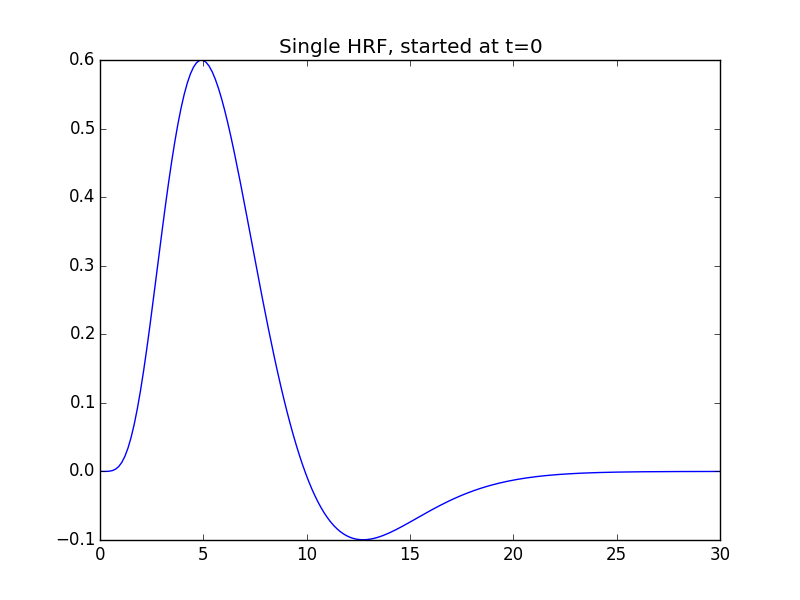
\includegraphics[width=.8\linewidth]{images/hrf_pattern.png} 
	\caption{$f$ (``Stablized Function'')}
	\label{fig:hrf}
\end{minipage}	
\quad
\begin{minipage}[b]{0.45\linewidth}
	\centering
	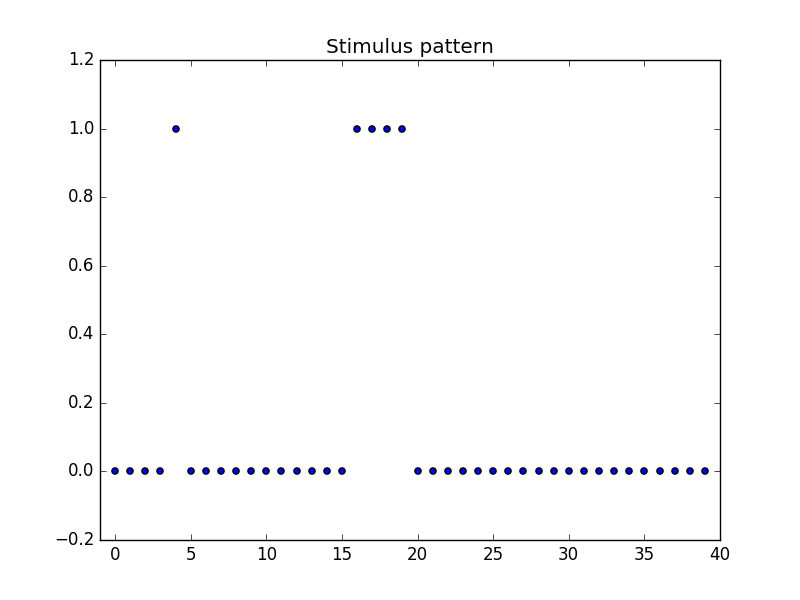
\includegraphics[width=.8\linewidth]{images/on_off_pattern.png} 
	\caption{$g'$ (``Moving function'')}
	\label{fig:on_off}
\end{minipage}
\end{figure}


\begin{figure}[ht]
	\centering
	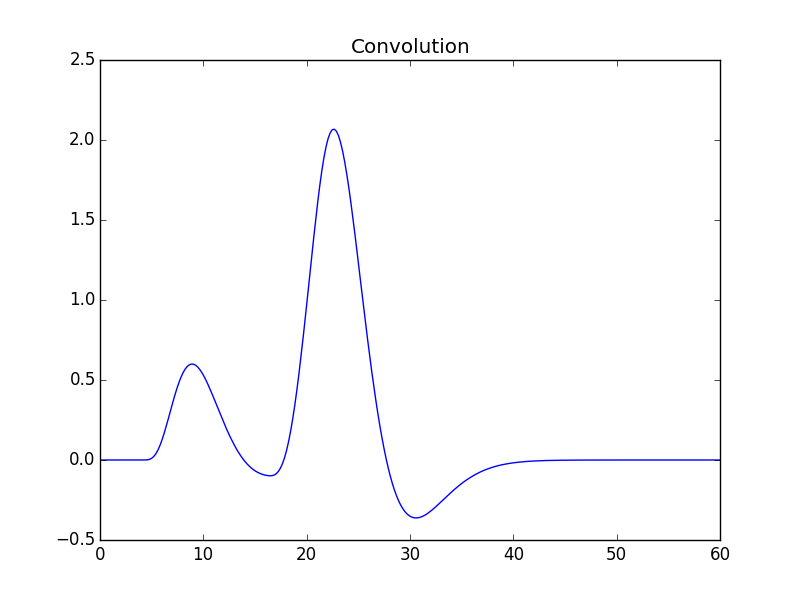
\includegraphics[width=.5\linewidth]{images/initial_convolved.png}
	\caption{convolution of $f$ and $g'$}
	\label{fig:convolve1}
\end{figure}



\subsection{Bring it back to Earth, and fMRI}

With this discrete approach to convolution between $f$ and $g'$, we can deal 
with our data. The $f$ is actually a common representation of the hemodynamic 
response, and the $g'$ is a good representation of the stimulation from an 
event-related trial \cite{brett2015course}. 

\section{Approach to our Specific Problem}

\subsection{Common Approach (\texttt{np.convolve})}

A common approach to convolve 2 functions in the way described above 
utilizes \texttt{np.convolve}, which uses fast fourier transforms for 
efficiency (it boils down to fewer computations using roots of unity). 
\texttt{np.convolve} assumes that the intervals between stimuli mirror the 
desired intervals between prediction intervals. It should be noted that 
\texttt{np} is a common notation for the \texttt{numpy} module in 
\texttt{python}.

\subsection{Moving beyond \texttt{np.convolve}, and needed improvements}

The reason motivating this appendix is that our data and needs fail to meet 
the assumption that the intervals are in equidistant. Especially in our case, 
there was not an easy route in terms of basic rounding to then correctly utilize 
\texttt{np.convolve}. All the following approaches improve on the basic 
\texttt{np.convolve} approach, but ultimately circle back to incorporating 
\texttt{np.convolve} for speed gains. 

\subsubsection{Our data/situation explained}
Our condition file (\texttt{cond1}) lists stimulus times for when the 
individual pumped the balloon but didn't pop it. For subject 001, the 
first 10 data points are as follows [Figure \ref{table:cond1}]:

\vspace{5mm}

\begin{figure}[ht]
\begin{center}
\begin{tabular}{|cccccccccc|}
  \hline
0.0671 &
2.1251 &
3.7681 &
5.6601 &
7.8673 &
9.3443 &
19.7831 &
22.0402 &
23.5837 &
25.1434 \\
 \hline

  \end{tabular}
   \caption{First 10 values for Sub 001, condition 1}
  \label{table:cond1}
\end{center}
\end{figure}
 
Clearly, this short time series doesn't align with scans that start at 
$t=0$ and occur every 2 seconds apart. As such, we had to go back to the 
drawing board to try to reproduce our expected hemodynamic reponse for the 
whole time course.



\subsubsection{Summary of Approaches}
Our first approach attempts to reproduce the theoretical rigor for our data. 
Our second approach tries to utilitize \texttt{np.convolve} by expanding the 
grid of desired results (thanks to advice from Jean-Baptiste Poline).




\subsubsection{Initial correction to represent theoretical idea}
To account for our data's lack of any easily identifiable grid structure 
between when a stimulus was recorded and when our scans occured (on the 
order of every 2 seconds), we went back to the theory of convolution and 
implemented code to recreate equation \ref{eq:math_discrete_final} directly. 
To do so, we also had to create a function that treated all discrete points 
of $f$, the stimulus reponse as potential starts of the hemodyamic response, 
multiplied by the actual value of $f$, as see in equation 
\ref{eq:code_convolve}:

\begin{equation} \label{eq:code_convolve}
r(t)= \sum_{i=1}^n g'_{i} f(t-t_i)
\end{equation}

where $g'_{i}$ is the value of $g'$ at $t_i$ (allowing for zeroes and varying 
non-zero value of $g'$).


\subsubsection{Matrix multiplication}
Equation \ref{eq:code_convolve}, rewritten below

$$r(t)= \sum_{i=1}^n g'_{i} f(t-t_i)$$

can be changed to a matrix multiplication problem:

\begin{equation} \label{eq:matrix_code_convolve}
r(t)=  g^*(t)^T f^*(t)
\end{equation}

where the $g^*$ is a vectorized function of $g'$ of $t$ as a scalar output and 
$f^*$ is the vector of $f$ values (irrespective of location, as the $t^*$ 
takes that into account).


\subsubsection{Utilization of FFT with \texttt{np.convolve}}
The ''theoretical'' solution lacked computation efficiency (although the 
matrix version increased speed by a lot), so we also approached the problem by 
creating a more dense grid between each scan (2 seconds apart). Then we rounded 
the actual times of the stimulus to meet this more finely scaled grid. This 
allowed us to utilize \texttt{np.convolve} with it's faster algorithms 
(using FFT), and then reduce back down to our 2 second grid.

We initially started with 30 slices in between each scan, but matrix 
multiplication actually beat this analysis, so we reduced the time cost by 1/2 
(with only 15 slices), and so little decline is accuracy.

This method does loose accuracy, but since the ideas behind this process don't 
really have very strong relationships to real life, a little accuracy loss is 
acceptable for speed.


%Needed references:
%Brett, Matthew and Poline, J-B  (2013). Convolution. Retrieved from 
% http://practical-neuroimaging.github.io/on_convolution.html

% Weissten, Eric W. ``Convolution''. From MathWorld - A Wolfram Web  Resource. 
% Retrieved from htt://mathworld.wolfram.com/Convolution.html

\bibliography{project}

\end{document}
